% Willkommen im Quelltext. :-)
%
% Diese „Bachelor-Arbeit“ wurde mit LaTeX erstellt. Sie kann sowohl
% als Vorlage für Ihre eigene Bachelor-Arbeit verwendet werden als
% auch als Einführung in das Arbeiten mit LaTeX.

% Lizenz: @@@ Tja ... CC-0? CC-BY-SA?

% Im Gegensatz zu What-You-See-Is-What-You-Get- (WYSIWYG-) Systemen
% wie z.B. Textverarbeitungsprogrammen im Office-Bereich, unterscheidet
% LaTeX zwei Versionen des Dokuments: den Quelltext und das compilierte
% Dokument.
%
%  * Der Quelltext ist diejenige Version, die man bearbeitet.
%    Dies geschieht mit einem beliebigen Texteditor, mit dem man
%    auch Computerprogramme schreiben würde. Die LaTeX-Sprache ist
%    eine Markup-Sprache – vergleichbar mit XML oder HTML –, stellt
%    dabei aber mächtigere Werkzeuge zur Verfügung bis hin zu echter
%    Programmierung (Verzweigungen, Schleifen).
%
%  * Durch Compilieren entsteht aus dem Quelltext das druckreife
%    Dokument – typischerweise eine PDF-Datei oder PostScript.
%    Für das vorliegende Dokument geschieht dies durch den Aufruf
%    „pdflatex hauptdatei.tex“ auf der Kommandozeile oder über einen
%    Menüpunkt.
%
% Dieses Dokument enthält zahl- und umfangreiche Kommentare (z.B.
% diesen), die eine kleine Einführung in die Arbeit mit LaTeX geben
% sollen. Kommentare werden mit einem Prozentzeichen eingeleitet und
% gehen jeweils bis zum Zeilenende.
%
% „Befehle“ (genauer: „Macros“) werden in LaTeX typischerweise
% durch einen Backslash eingeleitet und können daher zwischen dem
% eigentlichen Text stehen. Dennoch beginnt ein LaTeX-Dokument nicht
% direkt mit dem Text, sondern es hat einen Vorspann, in dem man
% Pakete einbinden und eigene Macros definieren kann.

% Die \documentclass-Zeile ist in der Regel die erste Zeile eines
% LaTeX-Dokuments. Sie definiert das allgemeine Dokumentenformat:
% Artikel, Bericht (mehrere Kapitel), Buch, Brief usw. Für eine
% Bachelor-Arbeit eignen sich Artikel- und Bericht-Formate. In
% diesem Beispiel verwenden wir das KOMA-Artikel-Format „scrartcl“;
% das entsprechende Bericht-Format heißt „scrreprt“.
%
% Die Optionen [in eckigen Klammern] bedeuten: Verwende A4-Papier,
% setze Gleichungen linksbündig stat zentriert, verwende 12-Punkt-
% statt 11-Punkt-Schrift, trenne die Kopfzeile durch einen
% horizontalen Strich vom Text.
%
\documentclass[a4paper,fleqn,12pt,headsepline]{scrartcl}

% Mit \usepackage bindet man Sammlungen nützlicher Befehle,
% sog. Pakete ein. Das graphicx-Paket stellt z.B. einen Befehl
% \includegraphics zur Verfügung, mit dem man (bei Verwendung von
% PDFLaTeX) Grafiken im PDF-, PNG- oder JPG-Format einbinden kann.
%
\usepackage{graphicx}
\usepackage{wrapfig}

% Umlaute und sonstige Sonderzeichen als UTF-8 direkt eingeben
\usepackage[utf8]{inputenc}
% Sprachpaket „reformierte deutsche Rechtschreibung“ einbinden
% (u.a. für Trennungen)
\usepackage[ngerman]{babel}	% Für Englische Berichte ausqwählen und auskommentieren
%\usepackage[english]{babel} 		% Für Englische Berichte ausqwählen und auskommentieren

% Zeichensätze und Zeichensatzkodierung auswählen
%
% Unten sind verschiedene Möglichkeiten aufgeführt, aber nur eine
% wird tatsächlich verwendet. Die anderen sind „auskommentiert“;
% um diese auszuprobieren, genügt es, Kommentarzeichen zu verschieben.
%
\usepackage[T1]{fontenc}
%
%\usepackage{fix-cm} % Standard-Schriftfamilie “Computer Modern” in einer flexibleren Variante verwenden
\usepackage{lmodern} % Schriftfamilie „Latin Modern“ (Erweiterung von „Computer Modern“) verwenden
%\usepackage{droid} % Schriftfamilie „Droid“ verwenden
%\usepackage{times} % „Times New Roman” als Serifenschrift verwenden
%\usepackage{librebaskerville} % „Libre Baskerville” als Serifenschrift verwenden
%\usepackage{libertine} % „Linux Libertine” als Serifenschrift verwenden
%\usepackage{fourier} % „Utopia Regular” als Serifenschrift verwenden
%\usepackage{fouriernc} % „New Century Schoolbook” als Serifenschrift verwenden
%\usepackage{tgschola} % „TeX Gyre Schola” als Serifenschrift verwenden
%\usepackage[scaled=0.95]{helvet} % leicht verkleinerte „Helvetica“ als Sans-Serif-Schrift verwenden
%
% Sans-Serif-Schrift als Standardschrift benutzen
%\renewcommand*\familydefault{\sfdefault}

% Wenn man Anführungszeichen unten und oben nicht von Hand eingeben
% will oder kann (z.B. „Test“), ermöglicht das csquotes-Paket u.a.,
% stattdessen \enquote{Test} zu schreiben.
%
%\usepackage[babel,german=quotes]{csquotes}	% Nur für deutsche berichte einkommentieren
% 

% Das float-Paket stellt erweiterte Möglichkeiten zur Plazierung von
% Abbildungen und sonstiger „gleitender“ Inhalte zur Verfügung.
%
\usepackage{float}

% Bilder mit „Bild“ anstatt mit „Abbildung“ bezeichnen
\renewcaptionname{ngerman}\figurename{Bild} % für deutsche Berichte inkommentiern nur 
%\figurename{Fig:}  		% nur für englische Verichte einmkommentieren 

% Das picins-Paket stellt Befehle zur Verfügung, Bilder in den Text
% zu integrieren und umfließen zu lassen.
%
%\usepackage{picins}

% Bilder, Tabellen usw. sind in LaTeX normalerweise „gleitend“,
% d.h., sie stehen nicht an einer bestimmten Stelle im Text, sondern
% z.B. oben auf der Seite. Wenn man Bilder usw. nicht gleiten läßt,
% sondern sie fest mit dem Text verbindet, ermöglicht dieses Paket,
% ihre Beschriftung (caption) dennoch im Abbildungsverzeichnis
% erscheinen zu lassen und darauf zu verweisen.
%
% Die hier verwendete KOMA-Version scrartlc des Artikel-Formats
% enthält bereits die in diesem Paket enthaltenen Befehle. Sie
% benötigen es daher nur, wenn Sie das Standard-Artikel-Format
% article verwenden.
% 
%\usepackage{capt-of}

% Paket für mehrseitige Tabellen
%\usepackage{longtable}

% Paket für Seitenrandabstände und Einstellung für Seitenränder
\usepackage{geometry}
\geometry{left=3.5cm, right=2cm, top=2.5cm, bottom=2cm}

% Paket für Kästchen mit Spezialeffekten (z.B. Schatten)
%\usepackage{fancybox}

% bricht lange URLs „schön“ um
\usepackage[hyphens,obeyspaces,spaces]{url}

% Paket für Textfarben
\usepackage{color}
\usepackage{xcolor}

% Zusätzliche mathematische Symbole importieren
\usepackage{amsmath}
\usepackage{amssymb}

% erzeugt Inhaltsverzeichnis mit Querverweisen zu den Kapiteln (PDF Version)
\usepackage[bookmarksnumbered,hyperfootnotes=false]{hyperref} 
\hypersetup{colorlinks,citecolor=black,linkcolor=black,urlcolor=black}

% neue Kopfzeilen mit dem fancyhdr-Paket erzeugen
\usepackage{fancyhdr} % Paket laden
\pagestyle{fancy} % eigener Seitenstil
\fancyhf{} % alle Kopf- und Fußzeilenfelder bereinigen
\fancyhead[L]{\nouppercase{\leftmark}} % Kopfzeile links
\fancyhead[C]{} % zentrierte Kopfzeile
\fancyhead[R]{\thepage} % Kopfzeile rechts
\renewcommand{\headrulewidth}{0.4pt} % obere Trennlinie

% Festlegung der Art der Zitierung auf die Havard-Methode: Abkürzung Autor + Jahr.
% Dieser Befehl gehört zum natbib-Paket.
%
\usepackage{natbib}
\bibliographystyle{apalike_german}

% keine Einrückung am Anfang eines Absatzes,
% stattdessen vertikal etwas Platz lassen
%
\usepackage{parskip}

% Paket zur Erweiterung der Tabellen-Befehle (tabular, array)
%\usepackage{array}

% Dieser Befehl würde den zusätzlichen Zwischenraum abschalten,
% den LaTeX normalerweise nach einem Punkt einfügt.
%\frenchspacing

% Paket für Zeilenabstand einbinden
%\usepackage{setspace}
% Dieser Befehl würde den Zeilenabstand auf „1,5“ einstellen
%\onehalfspacing

% Paket für Listings (z.B. Computerprogramme)
\usepackage{listings}
%
% Einstellungen für C-Quelltexte
%\lstset{numbers=left,
%        numberstyle=\tiny,
%        numbersep=5pt,
%        keywordstyle=\color{black}\bfseries,
%        stringstyle=\ttfamily,
%        showstringspaces=false,
%        basicstyle=\footnotesize,
%        captionpos=b}
%\lstset{language=c}
%
% Einstellungen für LaTeX-Quelltexte
\lstset{basicstyle=\ttfamily,
        language=tex}
        
\lstset{numbers=left,
        numberstyle=\tiny,
        basicstyle=\small,
        language=python}       

% Nomenklatur
%
% Paket einbinden
\usepackage{nomencl}
%
% Befehl „\nomenclature” alternativ als „\abk“ zur Verfügung stellen
\let\abk\nomenclature
%
% Deutsche Überschrift für Nomenklaturverzeichnis
\renewcommand{\nomname}{Nomenklatur} % nur für deutsche Berichte 
%
% Nomenklaturverzeichnis gestalten
% Raum, der den Abkürzungen zur Verfügung steht = 0.2 der Gesamtbreite
\setlength{\nomlabelwidth}{0.2\hsize}
% Zeilenabstände verkleinern
\setlength{\nomitemsep}{-\parsep}
\makenomenclature
% Erstellen von Unterteilungen in der Nomenklatur
\RequirePackage{ifthen}
\renewcommand{\nomgroup}[1]{%
 \ifthenelse{\equal{#1}{A}}{\item[\textbf{Abkürzungen}]\vspace*{1cm}}{%
    \ifthenelse{\equal{#1}{S}}{%
      \item[\textbf{Symbole}]\vspace*{1cm}}{}%
  }%
}


% Benutzte in Überschrift die gleiche Schriftart und Farbe wie im Text
\setkomafont{disposition}{\normalcolor\bfseries}

% Maßeinheit für picture-Grafiken
\setlength{\unitlength}{1cm}

%
% fuer Stichwortverzeichnis
\usepackage{makeidx}
% Stichwortverzeichnis erstellen
\makeindex
\renewcommand{\indexname}{Stichwortverzeichnis} % nur für deutsche Berichte 

%%%%%%%%%%%%%%%
% pgfplots und tikz
\usepackage{tikz}
\usepackage{pgfplots}
\pgfplotsset{compat=1.18}% hinzugefügt, ML 20130601

\usetikzlibrary{patterns}
\usetikzlibrary{datavisualization}
\usetikzlibrary{arrows}

\usepackage{gensymb}
\usepackage{booktabs}
\usepackage{longtable}
\usepackage{multirow}
\usepackage[toc,page]{appendix} % für englische Berichte


% Bildnummern aus Nummer des Abschnitts und laufender Nummer zusammensetzen
%
% Bei Verwendung eines Bericht-Formats (s.o.) geschieht dies
% automatisch mit der Kapitelnummer (\chapter – eine Ebene oberhalb
% von \section). Für das Artikel-Format machen wir es hier manuell.
%
\renewcommand{\thefigure}{\arabic{section}.\arabic{figure}}
\makeatletter\@addtoreset{figure}{section}\makeatother

% Gleichungsnummern aus Nummer des Abschnitts und laufender Nummer zusammensetzen
\renewcommand{\theequation}{\arabic{section}.\arabic{equation}}
\makeatletter\@addtoreset{equation}{section}\makeatother

% Tabellennummern aus Nummer des Abschnitts und laufender Nummer zusammensetzen
\renewcommand{\thetable}{\arabic{section}.\arabic{table}}
\makeatletter\@addtoreset{table}{section}\makeatother



% auf römische Seitenzahlen umschalten
%\pagenumbering{Roman}

% Mit \input wird eine selbst erstellte .tex-Datei eingebunden.
%
% „trennung.tex“ enthält ein (selbst erstelltes) Verzeichnis mit
% Trennhilfen für häufige Wörter, deren Silbentrennung von der
% Automatik nicht korrekt erkannt wird.
%
%hier müssen alle Wörter rein, welche Latex von sich auch nicht korrekt trennt bzw. bei denen man die genaue Trennung vorgeben möchte
\hyphenation{
Film-pro-du-zen-ten
Lux-em-burg
Soft-ware-bau-steins
zeit-in-ten-siv
wis-sen-schaft-li-chen
ent-spre-chend
}

% Mit \newcommand definieren wir einen neuen Befehl.
% Die 1 in eckigen Klammern bedeutet, daß der Befehl einen Parameter
% (bei Verwendung in geschweiften Klammern zu setzen) akzeptiert.
% Mit #1 nehmen wir auf diesen Parameter bezug.
%
% Der Befehl bewirkt, daß der Parameter in Sans-Serif-Schrift gesetzt wird.
%
% Beispiel für die Verwendung des Befehls: \file{hauptdatei.tex}
%
% Man könnte natürlich auch direkt \textsf{hauptdatei.tex} schreiben.
% Der neue Befehl hat aber den Vorteil, daß er markiert, was wir meinen
% und nicht, wie es aussehen soll. Konkret: Wenn wir uns im Nachhinein
% dafür entscheiden, Dateinamen doch nicht in Sans-Serif-Schrift, sondern
% z.B. kursiv zu setzen, muß dafür nur die Befehlsdefinition geändert werden
% – und nicht jede einzelne Stelle, an der der Befehl verwendet wird.
%
\newcommand{\file}[1]{\textsf{#1}}
\newcommand{\strong}[1]{\textbf{#1}}
\newcommand{\highlightRef}[2]{\href{#1}{\emph{\textbf{#2}}}}
\newcommand{\highlightFootCite}[2]{\emph{\textbf{#1}}}

% Mit \begin{document} endet der Vorspann, und das eigentliche
% Dokument beginnt.

\begin{document}
%
  % Titelseite
  %
  % Mit \newcommand definieren wir eigene Befehle – in diesem Fall
  % mit dem Zweck, Form und Inhalt zu trennen: In der Datei
  % „deckblatt.tex“ gestalten wir ein Deckblatt zur allgemeinen
  % Verwendung; für den konkreten Titel der Arbeit, Namen des Autors
  % usw. verwenden wir „Variablen“ \thetitle, \theauthor usw., die
  % wir hier vorab setzen.
  %
  \newcommand{\institutname}{  Institut für Mechatronik\\  und Fahrzeugtechnik}
%  \newcommand{\institutname}{  Institut für Informatik\\  und eingebettete Systeme}
  \newcommand{\thetitle}{Wirklich Aussagekräftiger\\ % Umbruch an sinnvollen Stellen manuell vornehmen
                         Titel}
  \newcommand{\theauthor}{Rene Kolling}
  \newcommand{\studentnumber}{017201445}
  \newcommand{\discipline}{Technische Informatik}
  \newcommand{\abschluss}{Bachelor of Engineering}
%  \newcommand{\abschluss}{Master of Engineering}
%  \newcommand{\dokumentname}{Dokumentation des KIS-Projekt-1 im Studiengang}
%  \newcommand{\dokumentname}{Dokumentation des KIS-Projekt-2 im Studiengang}
%  \newcommand{\dokumentname}{Dokumentation des KIS-Projekt-3 im Studiengang}
%  \newcommand{\dokumentname}{Dokumentation der Praxisphase im Studiengang}
  \newcommand{\dokumentname}{Softwareentwicklungsprojekt}
%  \newcommand{\dokumentname}{Master-Arbeit im Studiengang}
  \newcommand{\finaldate}{35.~Mai 2038}
 % Sperrvermerk, falls notwendig 
%%
\vspace*{10ex}

\begin{center}
\huge{\textbf{Sperrvermerk}}
\end{center}

\bigskip 


Die vorliegende Bachelor-Thesis mit dem Titel:

\begin{center}
\thetitle
\end{center}

beinhaltet interne und vertrauliche Informationen der Firma:

<Name und Anschrift der Firma>

Die Weitergabe des Inhalts der Arbeit und eventuell beiliegender Zeichnungen und Daten – im Ganzen oder in Teilen – ist bis zum 

<Datum, an dem der Sperrvermerk abläuft> 

grundsätzlich untersagt. Es dürfen keinerlei Kopien oder Abschriften – auch in digitaler Form – gefertigt werden.
Ausnahmen bedürfen der schriftlichen Genehmigung der o. g. Firma.
\bigskip 


Heiligenhaus, den 
%
\underline{\hspace*{2cm}} 
\underline{\hspace*{7cm}}\\
\hspace*{5.5cm}
<Unterschrift der/des Studierenden>

\clearpage
%
 \thispagestyle{empty}

\begin{minipage}{0.55\textwidth}
  Institut für Mechatronik\\
  und Fahrzeugtechnik
\end{minipage}\hfill
%
\includegraphics[height=2cm]{bilder/bologo} % Pixelgrafik-Version
\begin{picture}(0,0)(0,1.37) % Vektorgrafik-Version
  \put(-2.7,0.0){
\includegraphics[scale=1.06]{bilder/logo-hochschule-bochum-bo.pdf}}
  \put(-6.2,0.87){
\includegraphics[scale=0.545]{bilder/logo-hochschule-bochum-text.pdf}}
  \put(-6.2,-0.07){
\includegraphics[scale=0.635]{bilder/logo-hochschule-bochum-cvh-text.pdf}}
\end{picture}%

% freier Platz: 1/3 oben 
\vfill

\begin{center}
  % Die äußeren geschweiften Klammern begrenzen die Wirkung von \Huge.
  % Das \par am Ende ist notwendig, damit zum einen der Zeilenabstand
  % des \Huge-Textes angepaßt wird; zum anderen arbeitet \bigskip nicht
  % innerhalb von Textabsätzen, sondern außerhalb.
  {\Huge\textbf{\thetitle}\par}
  \bigskip\bigskip
  von\par
  \bigskip\bigskip
  {\Large\textbf{\theauthor}\par}
  \smallskip
  Matrikelnummer:~\studentnumber\par
  \bigskip\bigskip\bigskip
  \dokumentname\\
  \discipline\\
  zur Erlangung des akademischen Grades\\
  Bachelor of Engineering
\end{center}

% freier Platz: 2/3 unten
\vfill
\vfill
 
\begin{tabular}{ll}
  \textbf{Eingereicht am:} & \finaldate\\
  \\
  \textbf{1.~Prüfer:} & Prof.~Dr.-Ing.~Markus Lemmen \\
  \textbf{2.~Prüfer:} & M.~Sc.~Jan Weber 
\end{tabular}
 % Inhalt aus separater Datei lesen
%  \input{deckblatt-kis} % Inhalt aus separater Datei lesen

  % Abstract
  %
  % Mit \clearpage eröffnen wir eine neue Seite. Wenn sich noch
  % Bilder für den Beginn der nächsten Seite o.ä. im Speicher
  % befinden, soll LaTeX diese jetzt abarbeiten.
  \clearpage
  %
\pagenumbering{Roman}
\setcounter{page}{2}
  % Normalerweise wird bei einem neuen Abschnitt (\section{...}) die
  % Kopfzeile links automatisch auf den Namen dieses Abschnitts gesetzt.
  % Für das Abstract verwenden wir einen „stummen“ Abschnitt
  % (\section*{...}), bei dem dies nicht automatisch geschieht.
  % Mit dem folgenden Befehl setzen wir stattdessen die Kopfzeile
  % „von Hand“ auf „Abstract“.
  \fancyhead[L]{Abstract}
  %
  % Inhalt aus separater Datei lesen
  \section*{Abstract}

%Üblicherweise enthalten wissenschaftliche Artikel ein Abstract --
%  % "--" ist ein Gedankenstrich. Er ist länger und dünner als ein
%  % Bindestrich und hat eine andere Bedeutung.
%typischerweise von 100 bis 150 Wörtern,
%ohne Bilder und Literaturzitate und in einem Absatz.
%In dieser Vorlage gliedert sich das Abstract in diese Erläuterung
%sowie ein „echtes” Abstract, das nun als ein zweiter Absatz folgt.
%  % Die Anführungszeichen um „echtes“ sind UTF-8-Anführungszeichen unten und oben.
%  % Dasselbe Ergebnis kann man auch mit "`echtes"' oder \glqq{}echtes\grqq{}
%  % erreichen, bei Verwendung des csquotes-Pakets auch mit \enquote{echtes}.
%
%\LaTeX\ ist ein Textsatzsystem,
%  % Hinter Macros wie z.B. "\LaTeX" werden Leerzeichen normalerweise ignoriert.
%  % Damit dort trotzdem ein Leerzeichen erscheint, ergänzen wir dieses explizit
%  % durch den Macro "\ " – ein Backslash, gefolgt von einem Leerzeichen.
%das sich vor allem für die Erstellung wissenschaftlicher Arbeiten etabliert hat.
%Diese Vorlage demonstriert einige wichtige Grundlagen von \LaTeX\
%anhand einer Beispiel-Bachelor-Arbeit. Dies geschieht sowohl im
%fertigen Text (also diesem) als auch im \LaTeX-Quelltext,
%  % also diesem, ;-)
%typischerweise in Gestalt von Kommentaren.

Auf maximal einer Seite ist eine Kurzfassung der Arbeit anzugeben. Diese muss insbesondere die Motivation für die Arbeit und die zugrunde liegenden Fragestellungen, die gewählte Vorgehensweise und durchgeführten Aktivitäten sowie das Ergebnis der Arbeit enthalten. 
%Das Abstract wird im Internet veröffentlicht.



  % Inhaltsverzeichnis auf neuer Seite anzeigen
  \clearpage
  \fancyhead[L]{Inhaltsverszeichnis}
%  \fancyhead[L]{Table of Contents}
  \tableofcontents

  % Abkürzungsverzeichnis
  \clearpage
  \printnomenclature
  \fancyhead[L]{Nomenklatur} % Kopfzeile links
  %
  % Im Gegensatz zu anderen Abschnitten erscheint das
  % Abkürzungsverzeichnis nicht automatisch im Inhaltsverzeichnis.
  % Mit dem folgenden Befehl können wir es „von Hand“ ergänzen.
  %\addcontentsline{toc}{section}{Nomenklatur}

  % Abschnitt 1: Einleitung
  \clearpage
   %
  % Wenn wir oben die Kopfzeile links „von Hand“ gesetzt haben,
  % müssen wir sie jetzt auf „Automatik“ zurücksetzen.
  \fancyhead[L]{\nouppercase{\leftmark}}
  %
  % Wenn wir oben auf römische Seitenzahlen umgeschaltet haben,
  % können wir hier auf arabische Seitenzahlen zurückschalten und
  % den Seitenzähler zurücksetzen.
  %\pagenumbering{arabic}
  %
  % den eigentlichen Inhalt aus separater Datei einbinden
  \pagenumbering{arabic}
%
  % Mit \section{...} eröffnen wir einen neuen Abschnitt.
% Der Befehl setzt nicht nur den Text in einer größeren,
% fetten Schrift, sondern sorgt außerdem dafür, daß er im
% Inhaltsverzeichnis erscheint.
%
% Mit \label{...} erzeugen wir einen Bezeichner, mit dessen Hilfe
% wir später auf die Nummer des Abschnitts verweisen können (nämlich
% mit \ref{...}).
%
% Das Kommentarzeichen hinter „Übersicht“ dient dazu, ein
% Leerzeichen zwischen „Übersicht“ und dem \label-Befehl
% zu vermeiden, das andernfalls sichtbar würde – z.B. im
% Inhaltsverzeichnis.
%
\section{Einleitende Übersicht%
         \label{sec:Einleitung}}

Dieses Projekt befasst sich mit einem Modellfahrzeug das Automatisiert durch eine Strecke navigieren können soll. Dazu wird die Hardware größtenteils von der Firma Mdynamics zur Verfügung gestellt. 

Deshalb befasst sich diese Arbeit vorrangig mit der Software, die auf dem Framework von ROS (Robot Operating System) aufbaut sowie die Verarbeitung und Nutzbarmachung eines Beschleunigungssensors, im folgenden imu (inertial measurement unit) genannt. 
Ziel ist es, das Modellfahrzeug für den Wettbewerb des VDI - adc (autonomous driving challange) fit zu machen. Dazu soll es dem Fahrzeug möglich sein, diverse Disziplinen wie zum Beispiel das durchfahren einer Strecke, zu absolvieren. 
Um dieses Ziel zu erreichen werden Basisfunktionalitäten und eine Lineare- und Angulare-Geschwindigkeitsregelung erstellt. Für die Geschwindigkeitsregelung sollen die Odometrie des Fahrzeugs sowie die imu zusammen arbeiten. In der Theorie wäre es so möglich, eine Schlupfregelung zu erstellen damit das Fahrzeug maximal Beschleunigen und in Kurven an die Belastungsgrenzen der Reibung gehen kann um nicht aus der Kurve aus zu brechen. 
  \clearpage
  
  
  \section{Grundlagen/VDI-Racer %und Motivation der Arbeit
}
\label{sec:grundlagen}

VDI-Racer ist die interne Bezeichnung für das verwendete Modellfahrzeug. Dieses Fahrzeug soll technisch die Anforderungen erfüllen, an der Autonomous Driving Challenge\footnote{\url{https://www.vdi-adc.de/}} des VDI teil zu nehmen. Als Grundlage dient das MXcarkit (\cite{MXcarkitSpec}) der Firma Mdynamics\footnote{\url{https://mdynamix.de/en/about-us/}}.

\subsection{Stand der Technik}
Das Fahrzeug, sowie Teile der Software sind zu beginn dieses Projektes bereits vorhanden. In dem folgenden Abschnitt wird diese vorhandene Basis näher beleuchtet.

Der technische Stand hat sich im laufe des Projektes mehrmals geändert, ursprünglich war ROS melodic\footnote{\url{http://wiki.ros.org/Distributions}} (ROS 1) als Basis für das Projekt vorhanden. Darauf werden die meisten Tests, die in dieser Arbeit beschrieben sind, ausgeführt.

Aufgrund von Hardware-Änderungen und diversen anderen Projekten an diesem Fahrzeug, wurde das Fahrzeug später auf ROS2 galactic\footnote{\url{https://docs.ros.org/en/galactic/index.html}} migriert. Für das Projekt haben sich dadurch nur geringfügige Einflüsse ergeben, weshalb auf die neuere Struktur nicht näher eingegangen wird.


\begin{description}
    \item [Stand beginn des Projektes] --
    Zu beginn war das Fahrzeug bereits fahrtüchtig. Es war manuell steuerbar und es gab bereits die ersten Versuche einer autonomen Steuerung. Es war jedoch ein anderen Konzept umgesetzt. Ziel war es in diesem Konzept, dass Fahrzeug automatisch durch einen Raum navigieren zu lassen. Dazu sollte über den LIDAR eine Karte erstellt werden, in der sich das Fahrzeug über Anweisungen bewegen kann. Mit dem LIDAR konnte die eigene Position im Raum ermittelt werden und über einfache Befehle war es dann möglich an eine gegebene Stelle zu navigieren. 

    \item [Motivation] --
    Durch den bevorstehenden Wettbewerb des VDI hat sich das Konzept jedoch geändert. 
    Sollte das Fahrzeug sich vorher noch autark durch einen Raum bewegen, soll es nun dazu in der Lage sein verschiedene Disziplinen des VDI-Wettbewerbs zu meistern. 
    
    \item [Wettbewerb] --
    Der VDI-Wettbewerb ist in mehreren Disziplinen unterteilt, die durch ein Regelwerk definiert werden. 
    Eine dieser Disziplinen ist der Time Trial. 
    Ziel ist es in dieser Disziplin, dass das Fahrzeug auf einer Strecke, die durch Markierungen auf dem Boden abgegrenzt ist, möglichst viele Runden innerhalb der Zeit absolviert.\citep[11]{VDI-adc-Regelwerk} Dazu darf das Fahrzeug nicht ferngesteuert sein. 
    Eine Ausnahme dazu stellt der Startbefehl dar. Das Fahrzeug soll jegliche Entscheidungen ob zum Beispiel eine Gerade, eine Linkskurve oder eine Rechtskurve gefahren wird, selbständig treffen und danach handeln. Das Erfolgreiche absolvieren des Time Trails ist die größte treibende Kraft in diesem Projekt.
    
    Das Regelwerk differenziert für den Wettbewerb zwei Kategorien, den \textbf{VDI-Cup} und den \textbf{VDI-SuperCup} \citep[5]{VDI-adc-Regelwerk}. Beim \textbf{VDI Cup} ist die Hardware vorgegeben. Ausschließlich Softwarelösungen beeinflussen hier das Ergebnis. Die Hardware ist bei allen Fahrzeugen gleich oder gleichwertig. Der \textbf{VDI-Supercup} lässt bei der Hardware mehr Freiheitsgrade, hierbei ist es möglich, verschiedene Hardwarelösungen auszuprobieren um eventuell bessere, kostengünstigere oder einfach alternative Lösungen zu entwickeln.
\end{description}%

Prinzipiell ist es möglich mit dem Fahrzeug am VDI-Cup teil zu nehmen, da die Hardware von Mdynamics eigens für den Wettbewerb konzipiert wurde. Durch Anpassungen an der Hardware aus vorangegangenen Projekten und die Verwendung des Lidars wird 2022 vorerst der VDI-Supercup angestrebt. Für kommende Jahre soll der Fokus jedoch auf dem VDI-Cup liegen.

\bigskip 

%%%%%
\subsection{Aufbau / Komponenten des VDI-Racer}
\label{sec:VDI-Racer-Aufbau}

Das Fahrzeug besteht aus verschiedensten Aktoren und Sensoren. Diese Komponenten zusammen bilden das Grundgerüst für die gesamte Arbeit und besteht aus:

\begin{itemize}
    \item Chassis \& Karosserie
    \item Lenkung \& Servomotor
    \item Antrieb \& Motorsteuerung
    \item Stromversorgung Motor 2x LiPo Polymer Akkus 5200mAh 7,4V
    \item Fernsteuerung
    \item Jetson Xavier NX Developer kit (Computereinheit)
    \item Stromversorgung Jetson Powerbank
\end{itemize}

Die Sensorik des Fahrzeugs besteht aus:
\begin{description}
    \item [Inertial Measurement Unit MPU6050] (IMU) ist ein 6-Achsen Sensor-Modul. Aufgeteilt sind diese Achsen in 3-Achsen Beschleunigungssensor und 3-Achsen Gyroskop. Die Einheit kann durch die Fusion dieser Sensoren eine ROS-Sensormessage\footnote{\url{http://docs.ros.org/en/melodic/api/sensor_msgs/html/msg/Imu.html}} erstellen in der die Orientierung, die lineare Beschleunigung und die angulare Beschleunigung enthalten sind. Zudem besitzt die \strong{MPU6050} über eine Temperatursensor.

    \item [LIDAR] ist ein Laser-Sensor der sich um seine Achse rotiert und dabei den Abstand misst. Das Ergebnis ist eine 2D-Abstandsmessung um das Fahrzeug herum.
    
    \item [Kamera] 
    
    \item [Ultraschall-Sensoren] sind in der Lage, Objekte berührungslos zu erkennen und ihre Entfernung zum Sensor zu messen. Die Sensoren sind zwar mit dem MX-carkit mitgeliefert, jedoch noch nicht verbaut. Sie sollen später bei Disziplinen wie das Einparken helfen den Abstand zu Hindernissen zu messen.
    
    \item [Motorwinkel / Radwinkel / Drehzahl] werden von der Motorsteuerung genutzt um die Odometrie des Fahrzeugs zu bestimmen.
\end{description}
\cite{MXcarkitSpec}

\begin{figure}
  \begin{center}
  
    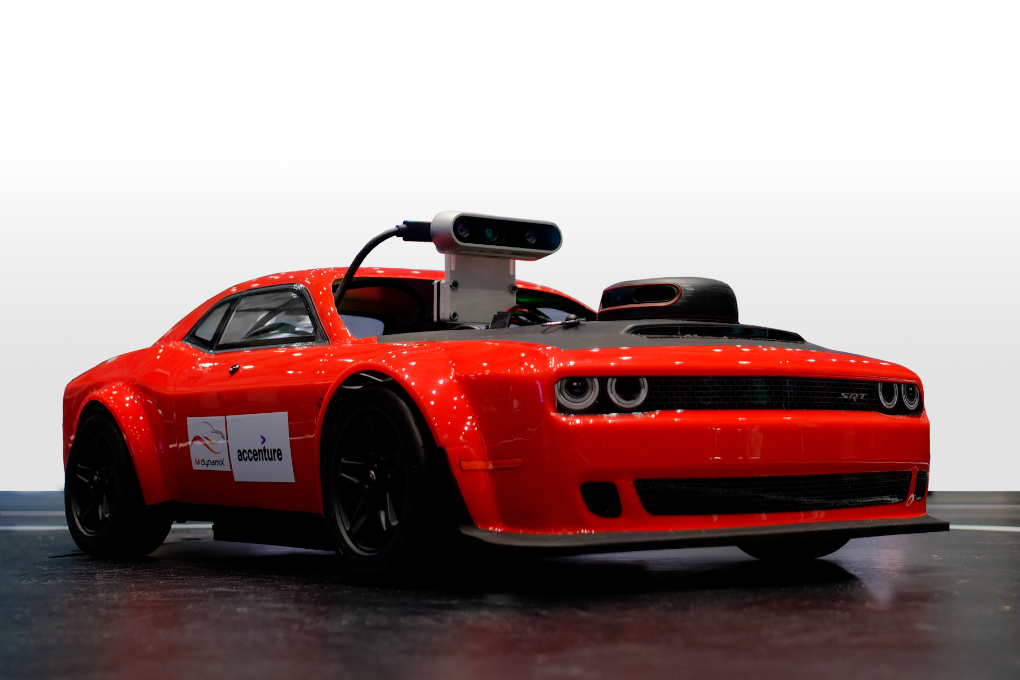
\includegraphics[width=\textwidth]{bilder/VDI-Racer.png}
  \caption{Bild des Fahrzeugs}
  \label{fig:vehicle}
  \end{center}
\end{figure}

\subsection{Grundlagen ROS}
\label{sec:grundlagen-ROS}
Die Software lief ursprünglich auf einem Jetson Xavier NX Computer mit einer ubuntu 18.04 Distribution von NVIDIA. NVDIIA stellt dazu das Jetpack bereit \footnote{\url{https://developer.nvidia.com/embedded/jetpack}}. Zwischenzeitlich hat sich das System geändert und mittlerweile läuft auf dem Computer die ubuntu 20.04LTS Distribution. 

Als Grundlage für die Software wird das Robot Operating System (ROS) verwendet. Dieses bietet schon viele Funktionalitäten und Schnittstellen um einen Roboter oder so wie hier ein Fahrzeug zu automatisieren. Dazu liefert das Framework ein Topic-Publisher/Subscriber-System, dieses ermöglicht einen Datenaustausch zwischen Programmen die sich untereinander nicht kennen müssen. Sie müssen sich nur bei ROS anmelden. Bevor die Programme Nachrichten nutzen können, müssen sie sich lediglich auf eine Syntax der Nachricht geeinigt haben. Dazu bietet ROS schon vordefinierte Nachrichten an, wie zum Beispiel float32\footnote{\url{http://docs.ros.org/en/lunar/api/std_msgs/html/msg/Float32.html}}. 

In der Dokumentation von ROS auf der Wiki-Seite heißt es ``ROS is an open-source, meta-operating system for your robot. It provides the services you would expect from an operating system, including hardware abstraction, low-level device control, implementation of commonly-used functionality, message-passing between processes, and package management. It also provides tools and libraries for obtaining, building, writing, and running code across multiple computers.''
\cite{ROS-Wiki}

\subsection{ ROS-Pakete }
\label{sec:ROS-Pakete}
ROS teilt die einzelnen Module und Funktionalitäten in Pakete auf. Jedes Paket soll dabei eine Aufgabe übernehmen wie zum Beispiel das ansteuern der Motorsteuerung. Diese Informationen werden dann über Topics mit einander getauscht. 
Einige dieser Pakete waren schon vor Beginn des Projektes lauffähig, da Sie in vorangegangenen Projekten erstellt oder eingebunden wurden und bieten einige Funktionalitäten. 

\begin{description}
    \item [vesc] 
    -- Hier steckt die \strong{Motorsteuerung} drin. Dieses Paket erlaubt es, Information an die Motorsteuerung zu senden und zu empfangen. Zudem bietet das Paket mehrere kleinere Nodes, wie zum Beispiel die Übersetzung eines Ackermann-Befehls\footnote{Als AckermannDrive wird im Englischen die Achsschenkellenkung bezeichnet. Der Ackermann-Befehl besteht aus einem Lenk-Winkel, der Geschwindigkeit und noch weiteren Werten. \url{http://docs.ros.org/en/jade/api/ackermann_msgs/html/msg/AckermannDrive.html}} in einen Lenkwinkel für den Servo. Auch die Odometrie wird von diesem Paket geliefert und kann als Topic subscribed werden.
    \item [rc-receiver] 
    -- Das RC-Receiver Paket liefert die Daten der \strong{Fernsteuerung} als Topic. Hierdurch kann das Fahrzeug manuell gesteuert werden. Zudem kann die Fernsteuerung verwendet werden, um einen Modus um zu schalten. 
    \item [mpu6050serial\_to\_imu] 
    \label{item:mpu6050}
    -- Dieses Paket bietet einen Node der den Arduino, an dem eine \strong{IMU} des Typs MPU6050 verbaut ist, ausließt. Zudem erstellt er aus den Daten zwei Topics die von anderen Nodes abgehört (Subscribed) werden können. Einmal die Positions- und Rotationsdaten selbst und die Temperatur werden versendet.
    \item [rplidar] 
    -- Das LIDAR Paket für ROS ist ebenfalls bereits erstellt und liefert eine Punktewolke über einen Topic. Das LIDAR kann den umgebenden Raum in einer 2-Dimensionalen Ansicht darstellen. Zusammen mit anderen Positionsermittelnden Sensoren wie der IMU und der Odometrie kann so die Position im Raum gefunden werden solange eine Karte verfügbar ist.
    %Zusammen mit einer Einschränkung des Winkels wurde dieses Modul lediglich dazu verwendet, den Abstand zu einem Hindernis vor dem Fahrzeug zu messen und ggf. das Fahrzeug zu stoppen. 
\end{description}

Um nun das Fahrzeug auf den Wettbewerb anzupassen, werden diese Module genutzt. Jedoch werden auch neue Pakete erstellt oder sogar bestehende Pakete angepasst.

%\subsection{ \textcolor{red}{IMU }} 

\subsection{Grundlagen Odometrie}
Die Odometrie ist eine Abschätzung der zurückgelegten Strecke. Um diese Abschätzung machen zu können, nutzt Sie die Umdrehungen des Motors. Diese werden von einem Sensor an die Motorsteuerung übergeben. Durch ein paar festgelegte Parameter wie der Raddurchmesser und der Achsabstand kann so eine recht genaue Abschätzung des linearen Anteils, aber auch eine grobe Schätzung des angularen Anteils der Strecke erstellt werden.  Das Paket \strong{vesc} hat dazu bereits ein Skript das aus der Motorsteuerung diese Werte als Topic hinterlegt, damit andere Skripte darauf zugreifen können.

  \clearpage
  \section{SW-Konzeption sowie Basisfunktionalitäten}
\label{sec:konzeption-kommunikation}
%
Das Konzept besteht aus drei Schichten. Eine dieser Schichten ist die Geschwindigkeitsregelung. Zudem gibt es die Kameraverarbeitung und die Trajektorienplanung. 
Zusammen %sollen 
bieten sie die Grundlage für das Fahrzeug, damit es dazu in der Lage ist, eine Strecke entlang zu fahren die durch weiße Linien begrenzt ist.

\begin{wrapfigure}[]{R}{0.4\textwidth}
    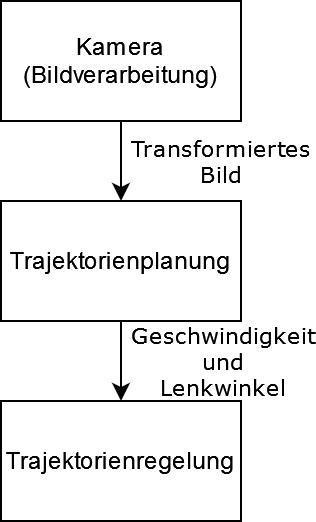
\includegraphics[width=0.4\textwidth]{bilder/DreiSchichten.png}
    \caption{Das Konzept in drei \\ Schichten unterteilt%
             \label{fig:dreiSchichten}}
\end{wrapfigure}

\begin{description}
    \item [Die Kameraverarbeitung]
    gibt ein bereits vorverarbeites, transformiertes Bild vor.
    \item [Die Trajektorienplanung]
    nimmt das Bild aus der Kameraverarbeitung und erstellt darin eine Trajektorie die eine Geschwindigkeit und eine Fahrtrichtung vorgibt.
    \item [Die Geschwindigkeitsregelung]
    bekommt die SOLL-Geschwindigkeit und den SOLL-Lenkwinkel von der Trajektorienplanung und regelt die IST-werte ein. 
\end{description}

Der Teil dieser Arbeit beschäftigt sich vor allem mit der Geschwindigkeitsregelung und anderen Basisfunktionalitäten. 
Der Geschwindigkeitsregler soll auf Basis der durch die Radodometrie gemessenen Radgeschwindigkeit und der durch die IMU gemessenen Beschleunigung die Geschwindigkeit des Fahrzeuges regeln. Die Implementierung der Regelung benötigt Vorarbeit denn die Odometrie des Fahrzeugs gibt eine Geschwindigkeit an, die IMU eine Beschleunigung. 
Damit nun beide Signale im Bezug zueinander genommen werden können muss entweder die Geschwindigkeit der Odometrie differenziert werden oder die Beschleunigung der Imu integriert. 
Beide Ansätze werden in dieser Dokumentation verfolgt und auf ihre Eignung getestet. Zuvor wurden jedoch ein paar Tests, mit der Imu und der Odometrie gemacht. 
Das Signal der Imu ist noch mit einer der Gravitationsbeschleunigung behaftet und zudem liegt das Koordinatensystem des Beschleunigungssensor nicht parallel dem des Fahrzeugs, näheres dazu in Abschnitt \ref{sec:imu}. 

\subsubsection{Konzept der Geschwindigkeitsregelung}
Die Regelung soll als Eingangssignal eine SOLL-Geschwindigkeit $v_{soll}$ von der Trajektorienplanung bekommen. Die Odometrie liefert eine Radgeschwindigkeit $v_{rad}$. Aus der Differenz von $v_{soll}$ und $v_{rad}$ lässt sich eine Regelabweichung $e$ bestimmen. Wenn die Die Differenz zwischen der Odometrie und den Werten der Imu sollen einen IST-Schlupf erzeugen.

\textcolor{red}{Wenn Sie da eine Regelung vornehmen wollen stellt sich die Frage: Was davon ist das Soll-Signal und was ist das IST-Signal von Geschwindigkeit und Beschleunigung...??? Für mich sind bis zu diesem Punkt in der Doku das jeweils \glqq{}Mess-Signale / Ist-Signale\grqq{}...! Für eine Regelung fehlt also nach wie vor eine Soll-Vorgabe...!}

\begin{figure}
    \centering
    \hspace*{-0.4cm}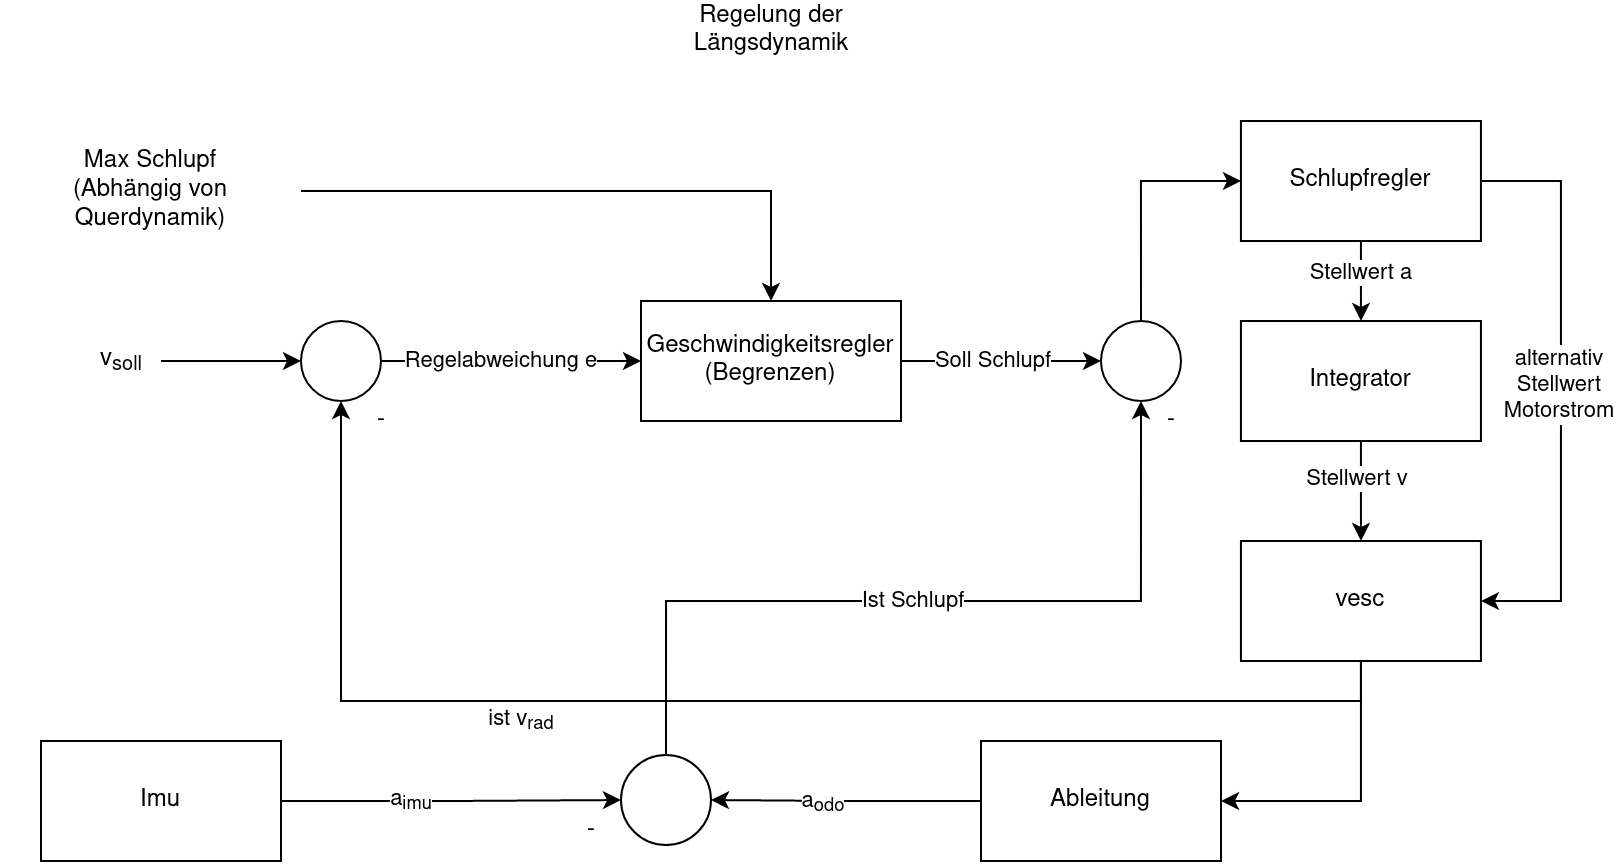
\includegraphics[width=1.05\textwidth]{bilder/SEP-Plan.png}
    \caption{Diagramm der Regelung}
    \label{fig:diagramRegelung}
\end{figure}

\subsection{Verbindung ROS Systeme}
In ROS 1 ist es noch notwendig ein paar Variablen im Terminal zu exportieren damit sich zwei Systeme im selben Netzwerk verbinden können.

Dazu stellt diese Dokumentation ein Skript zur Verfügung, um den Laptop mit dem Jetson, dem Computer des Autos, zu verbinden; das sogenannte  ROS-Master/Slave System. 
Mit Hilfe des Skripts gelingt es Skripte an einem anderen Rechner/System zu schreiben und zu starten.
%Dazu wurde ein kleines Skript geschrieben um den Laptop mit dem Jetson, der Computer des Autos, zu verbinden. (ROS-
%Master/Slave System)
%Dadurch können Skripte an einem anderen System geschrieben und gestartet werden. 
%Sind -- z.B. bei einem Wettbewerb / Rennen -- häufiger kleinere Änderungen vorzunehmen, so steht mehr (dezentralisierte) Rechenleistung für diese Aufgabe zur Verfügung 
%kann auf mehr Rechenleistung zurückgegriffen werden und diese müssen dann 

\subsection{Skripte}
Für alle erstellten Tests und Funktionen gibt es jeweils die folgenden Skripte.

\begin{description}
\item[move\_base.py]
ist ein Skript dass das Fahrzeug linear bewegt.
Dieses Skript wartet auf ein Signal das entweder 0 ist um zu stoppen oder 1 um
mit einer vorher definierten Geschwindigkeit geradeaus zu fahren.
Dieses Skript ermöglicht einfache Tests für die Beschleunigungs- und Geschwindigkeitsmessung.

\item[imuorientation.py]
ist ein Skript dass die Werte der IMU als Durchschnittswerte in der Konsole ausgibt. Als Input dient nutzt das Programm den Topic der IMU\footnote{\url{http://docs.ros.org/en/melodic/api/sensor_msgs/html/msg/Imu.html}}. Das Skript errechnet die Durchschnittswerte über mehrere Zyklen, so soll verhindert werden das Ausreißer zu viel Einfluss auf das Ergebnis haben. Nach einer vorgegebenen Zeit stoppt das Programm und gibt die Werte in der Konsole aus. Die Ausgabe besteht dann aus:
\begin{itemize}
    \item xMean, yMean zMean
    \item orientationRollMean, orientationPitchMean, orientationYawMean
    \item amountAccelerationMean
\end{itemize}
Besonders interessant zum Kalibrieren ist hier der Wert \strong{amountAccelerationMean}, er gibt den Betrag des Beschleunigungsvektor an.  
Das Ergebnis dieses Vektors sollte stets die Erdbeschleunigung sein. Durch empirische Versuche wurden so Ungereimtheiten mit der Kalibrierung der IMU behoben. Weiter Informationen zur Kalibrierung in Abschnitt \ref{sec:KalibrierungImu}.

\item[imuTestWithRemovingGravity.py]
ist analaog zu dem \strong{imuorientation.py} Skript, zudem entfernt es noch die Erdbeschleunigung aus den Daten. Das Resultat muss dann 0 ergeben. Dazu verwendet das Skript Quaternionen-Multiplikation. 

\lstinputlisting[language=Python, linerange={71-78,81-92,106-112}]{skripte/imutestWithRemovingGravity.py}

Dadurch das 6-Achsen durch die IMU gegeben sind, die Beschleunigung und die Orientierung zum Erdkoordinatensystem, kann durch die Anwendung von Quaternionen-Multiplikation das Koordinatensystem auf das Erdkoordinatensystem transformiert werden. Anschließend muss nur die Gravitation als Vektor abgezogen werden und bei Bedarf das Koordinatensystem wieder zurück transformiert werden. Dieses Skript diente vor allem dazu, zu Testen wie die Erdbeschleunigung raus gerechnet werden kann. Die Ergebnisse dieses Skriptes dienten zur Vorlage des \strong{remove\_gravity\_from\_imu.py} und anschließend des \strong{RemoveGravityFromImu.cpp} Skripts.

\item[remove\_gravity\_from\_imu.py] erbt von \strong{imuorientation.py} teile des codes. Dieses Skript ist in der 


-Diverse Skripte Tests mit der IMU und der Odometrie durch zu führen
-Einmal wurde das Signal der IMU Integriert um aus der Beschleunigung eine Geschwindigkeit zu bekommen (Hier muss natürlich deutlich mehr Inhalt und Referenzen
rein.)
-Zum Schluss wurde das Signal der Odometrie Differenziert um aus der Geschwindigkeit
der Odometrie eine Beschleunigung zu bekommen. (Das war analog zum anderen und
hat deutlich weniger Aufwand gekostet, könnte natürlich aber auch weiter ausgeführt
werden)

\end{description}

\subsection{imu}
\label{sec:imu}
Wie in Abschnitt \ref{sec:VDI-Racer-Aufbau} beschrieben, besteht eine IMU aus mehreren Sensoren, die Fusioniert und Ausgewertet die Orientierung, lineare sowie angulare Beschleunigung ergeben. Die IMU gibt die tatsächliche Beschleunigung des Fahrzeugs wider. Sie kann in einem Regelkreis dazu verwendet werden, die SOLL-Beschleunigung/Geschwindigkeit mit den Werten der IMU zu vergleichen, um dann eine Entscheidung zu treffen, ob die Beschleunigung zu stark oder zu schwach ist für den derzeitigen Untergrund. So soll das durchrutschen der Reifen vermieden werden.

\subsubsection{Kalibrierung}
\label{sec:KalibrierungImu}
Eine Kalibrierung des Sensors ist unerlässlich, da durch die Fertigung stets Unterschiede zwischen jeden Sensor bestehen. Für die Kalibrierung ist das Skript verantwortlich das auf dem Arduino läuft, dieses wird bereits von dem \strong{mpu6050\_serial\_to\_imu} Paket bereitgestellt. Das Sript ist jedoch so geschrieben, das es nach dem Verbinden mit dem Rechner die IMU jedes mal automatisch neu Kalibriert. Das führt zu einer immer anderen Kalibrierung, die eventuell nicht gewünscht ist. Es soll verhindert werden das, sollte sich die IMU während der Fahrt neu verbinden, die Kalibrierung in einer Bewegung statt findet, oder die Lage des Fahrzeugs sich ändert. 

Das bedeutet, dass die Kalibrierung manuell stattfindet. Dazu werden die Werte aus der automatischen Kalibrierung genommen und in den Code fest implementiert. Das \strong{imuorientation.py} Skript hilft dabei, die Kalibrierung zu überprüfen. Durch Systematisches auswerten der Achsen indem die IMU entweder Horizontal, Vertikal oder Beides positioniert wird

\subsubsection{Probleme und Hürden}
\label{sec:imu-probleme}
Die meisten Sensoren sind mit einem Rauschen behaftet oder führen gerade an Extrempunkten zu unerwünschten Verhalten. Auch die IMU hat diese Probleme, weshalb der Ansatz die Beschleunigungswerte der IMU zu nutzen um eine Geschwindigkeit zu erhalten, zu einer stetig steigenden (oder abnehmenden) Geschwindigkeit führt. Diesen Effekt nennt man bei Beschleunigungssensoren drift. Der Drift führt dazu, das der Beschleunigungssensor immer eine kleine Kraft in eine beliebige Richtung erfährt, ob er nun Still liegt oder nicht. Durch das Kalibrieren wird dieser Drift so weit es geht reduziert. Jedoch entsteht dieser drift vor allem durch die Erdanziehung, die eine konstante Kraft auf den Sensor ausübt. Damit diese Kraft möglichst keine oder nur geringe Auswirkungen auf das Ergebnis hat, wird sie aus den Messwerten entfernt. 

Das \strong{gravity\_from\_imu\_remover.cpp} Skript ist eigens dafür verantwortlich, die Gravitation aus der IMU raus zu rechnen. Es hört auf das Topic der IMU, rechnet die Erdbeschleunigung als Vektor \begin{equation}
    \vec g = \left(\begin{array}{c} 0 \\ 0 \\ 9.81 \end{array}\right)
\end{equation}
raus und versendet dann die eigenen Daten wieder als Topic und stellt die Daten damit anderen Programmen zur Verfügung. 

\begin{figure}
    \centering
%    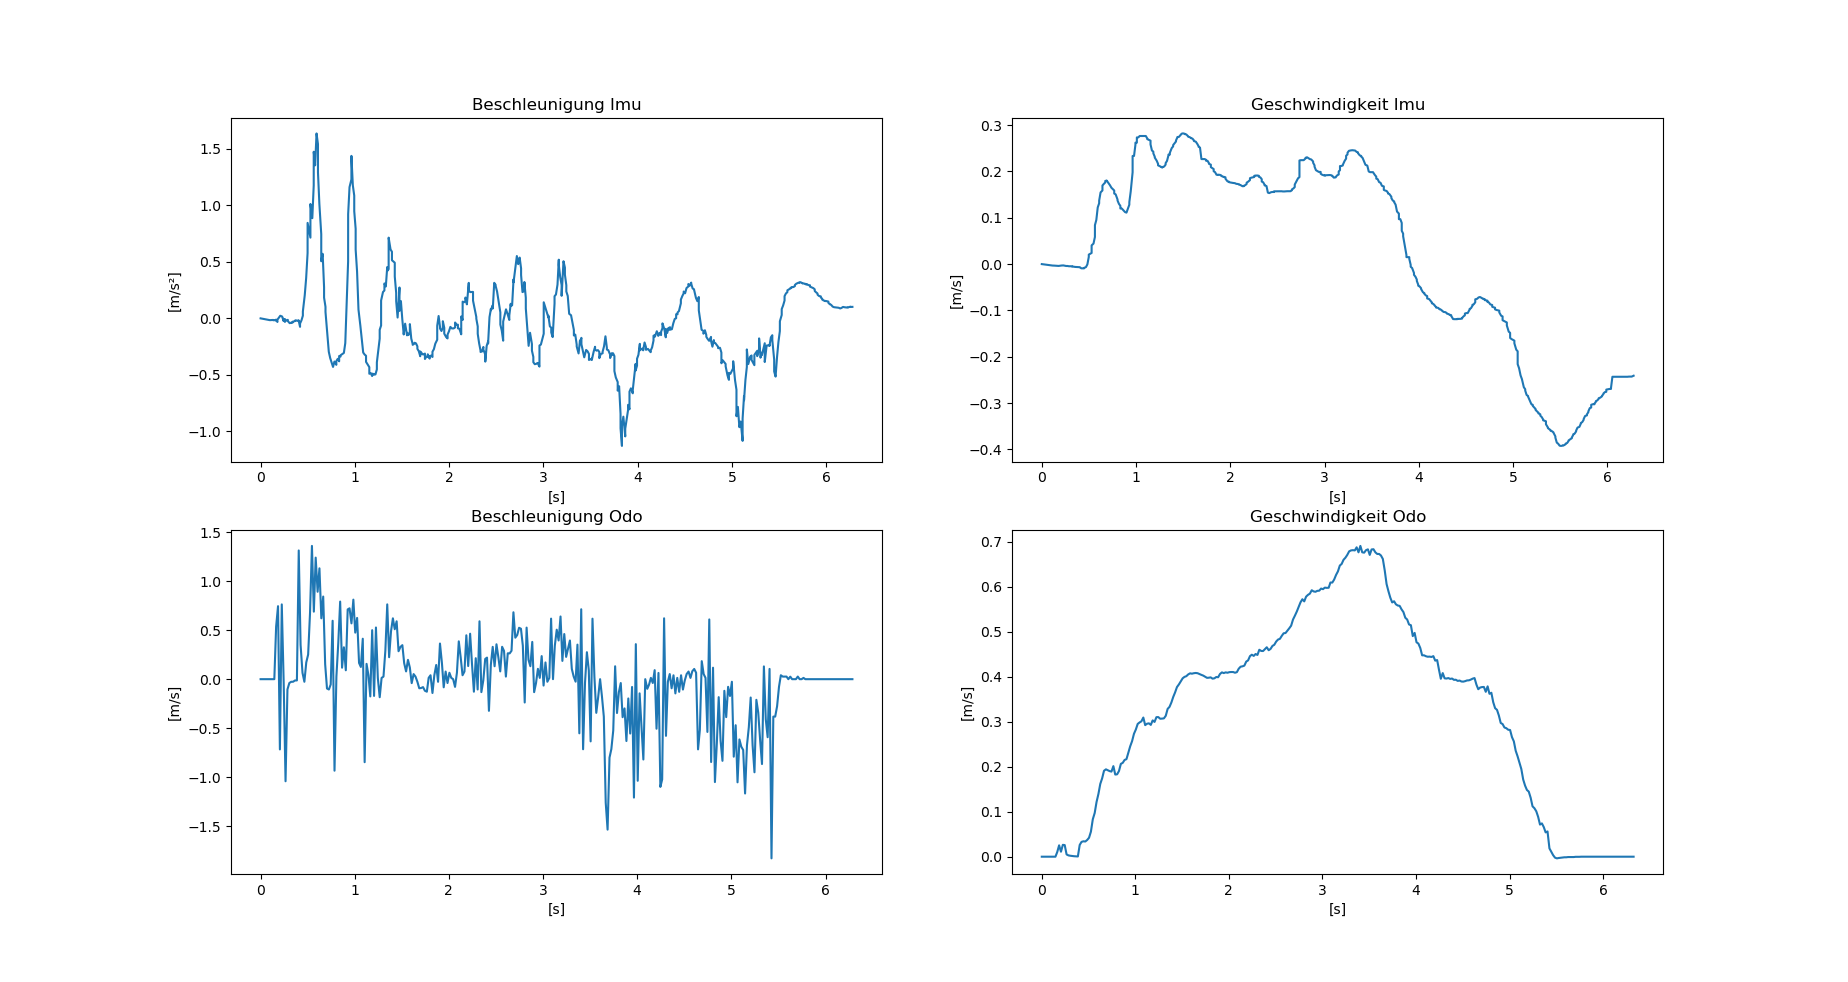
\includegraphics[width=\textwidth]{bilder/23AprImuOdoBeschlGeschw.png}
    \hspace*{-2cm}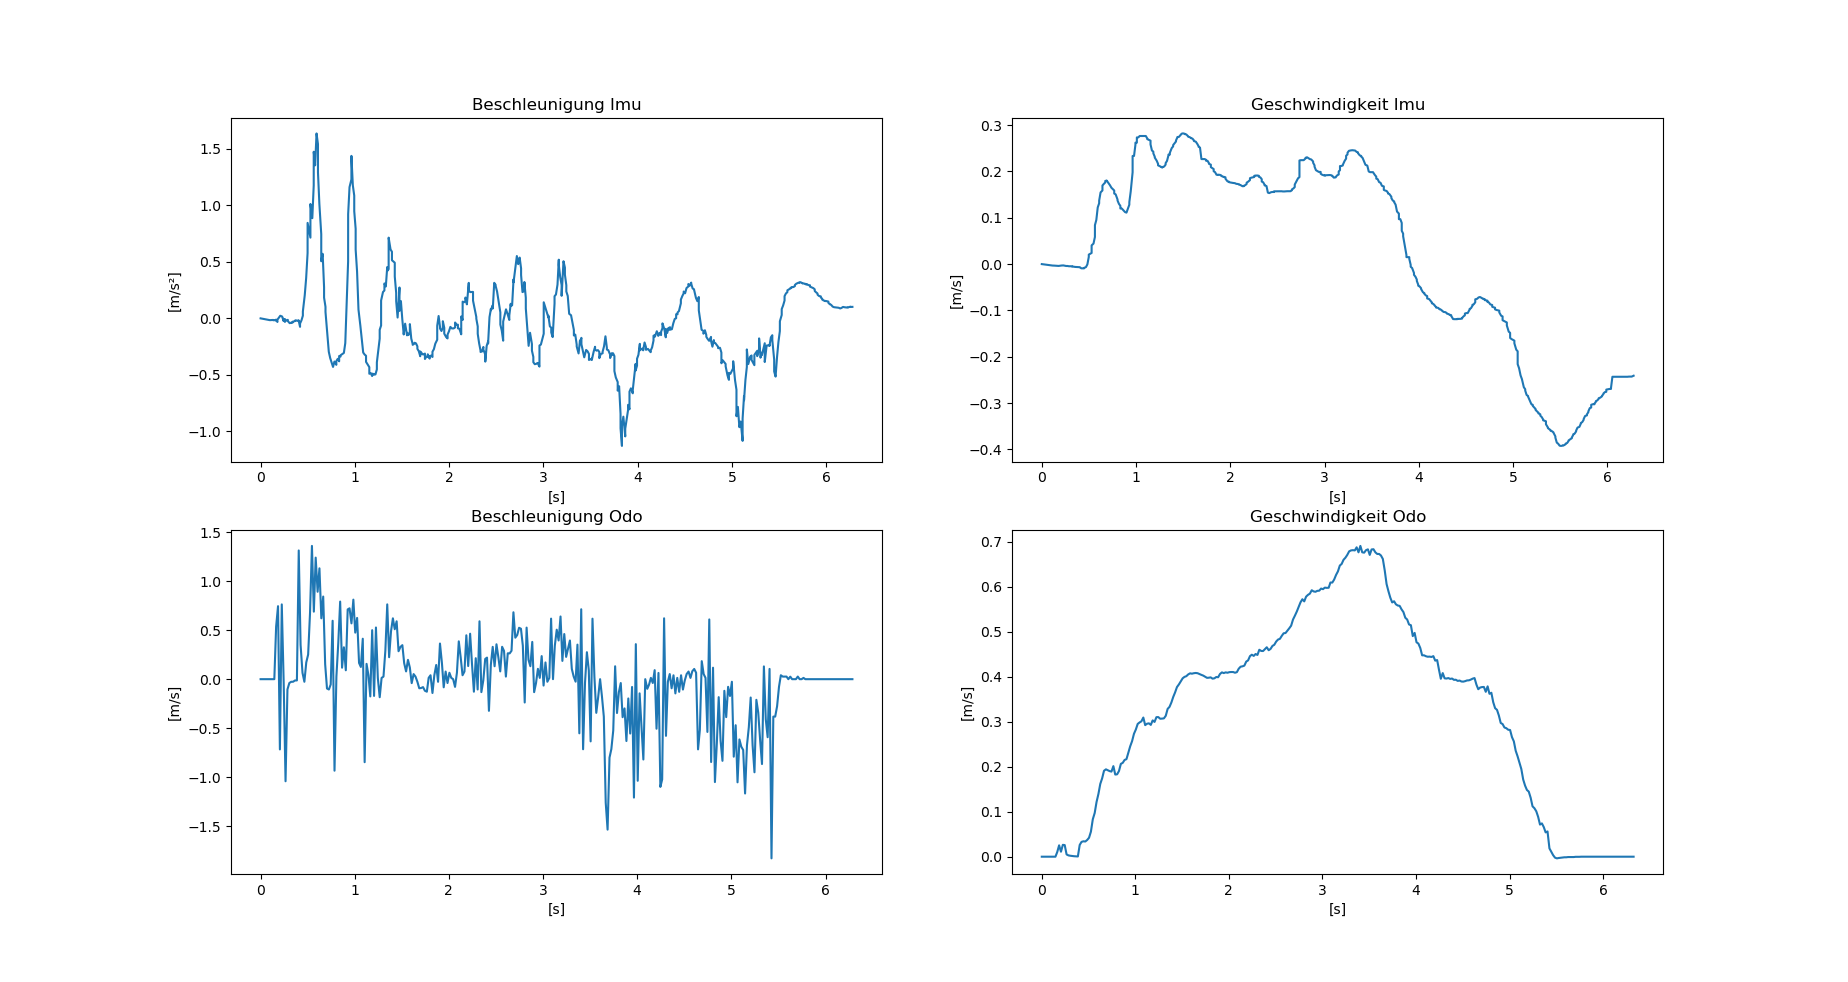
\includegraphics[width=1.25\linewidth]{bilder/23AprImuOdoBeschlGeschw.png}
    \caption{Einzelne Diagramme der Beschleunigung sowie der Geschwindigkeiten}
    \label{fig:diagramAprImuOdoBeschlGeschw}
\end{figure}

Das Problem wird deutlicher in Bild \ref{fig:diagramAprImuOdoBeschlGeschw}. In der Grafik oben rechts ist das Integrierte Signal der IMU. Obwohl das Fahrzeug, wie in der Ansicht der Odometrie unten rechts klar wird, steht, zeigt die IMU eine negative Geschwindigkeit an. Das Signal der Beschleunigung sieht dagegen zwar deutlich Chaotischer aus, offenbart jedoch zwischen Sekunde 5 und 6, dass die Odometrie und die IMU gerade in Extremen werten nicht gleich sind. Tatsächlich drehen die Reifen sich in diesem Szenario durch und die Beschleunigung der Odometrie zeigt nicht die tatsächliche Beschleunigung des Fahrzeugs, sondern nur die erwartete Beschleunigung aufgrund der Geschwindigkeit der Reifen. 

Der Aufbau eines Reglers kann erst stattfinden, wenn die Software diesen Werten vertrauen kann. Damit ist gemeint, dass die Überprüfung der Werte unerlässlich ist. 

\begin{lstlisting}
    sec: 1672855594
    nanosec: 699926525
    sec: 1672855594
    nanosec: 715770401
    sec: 1672855594
    nanosec: 731787777
    sec: 1672855594
    nanosec: 731886526
    sec: 1672855594
    nanosec: 747749124
    sec: 1672855594
    nanosec: 764142540
    sec: 1672855594
    nanosec: 764315234
    sec: 1672855594
    nanosec: 779952251
\end{lstlisting}

Zudem ist das \strong{imu\_transformer} Paket, das es von ROS gestellt gibt, dazu in der Lage die IMU Software-Seitig zu drehen. Sodass sie mit der x-Achse nach vorne zeigt und die z-Achse orthogonal vom Boden weg zeigt. Hierdurch ist es einfacher für Menschen, Lineare Kräfte von Angularen zu Unterscheiden.

\begin{figure}
    \centering
    \hspace*{-2cm}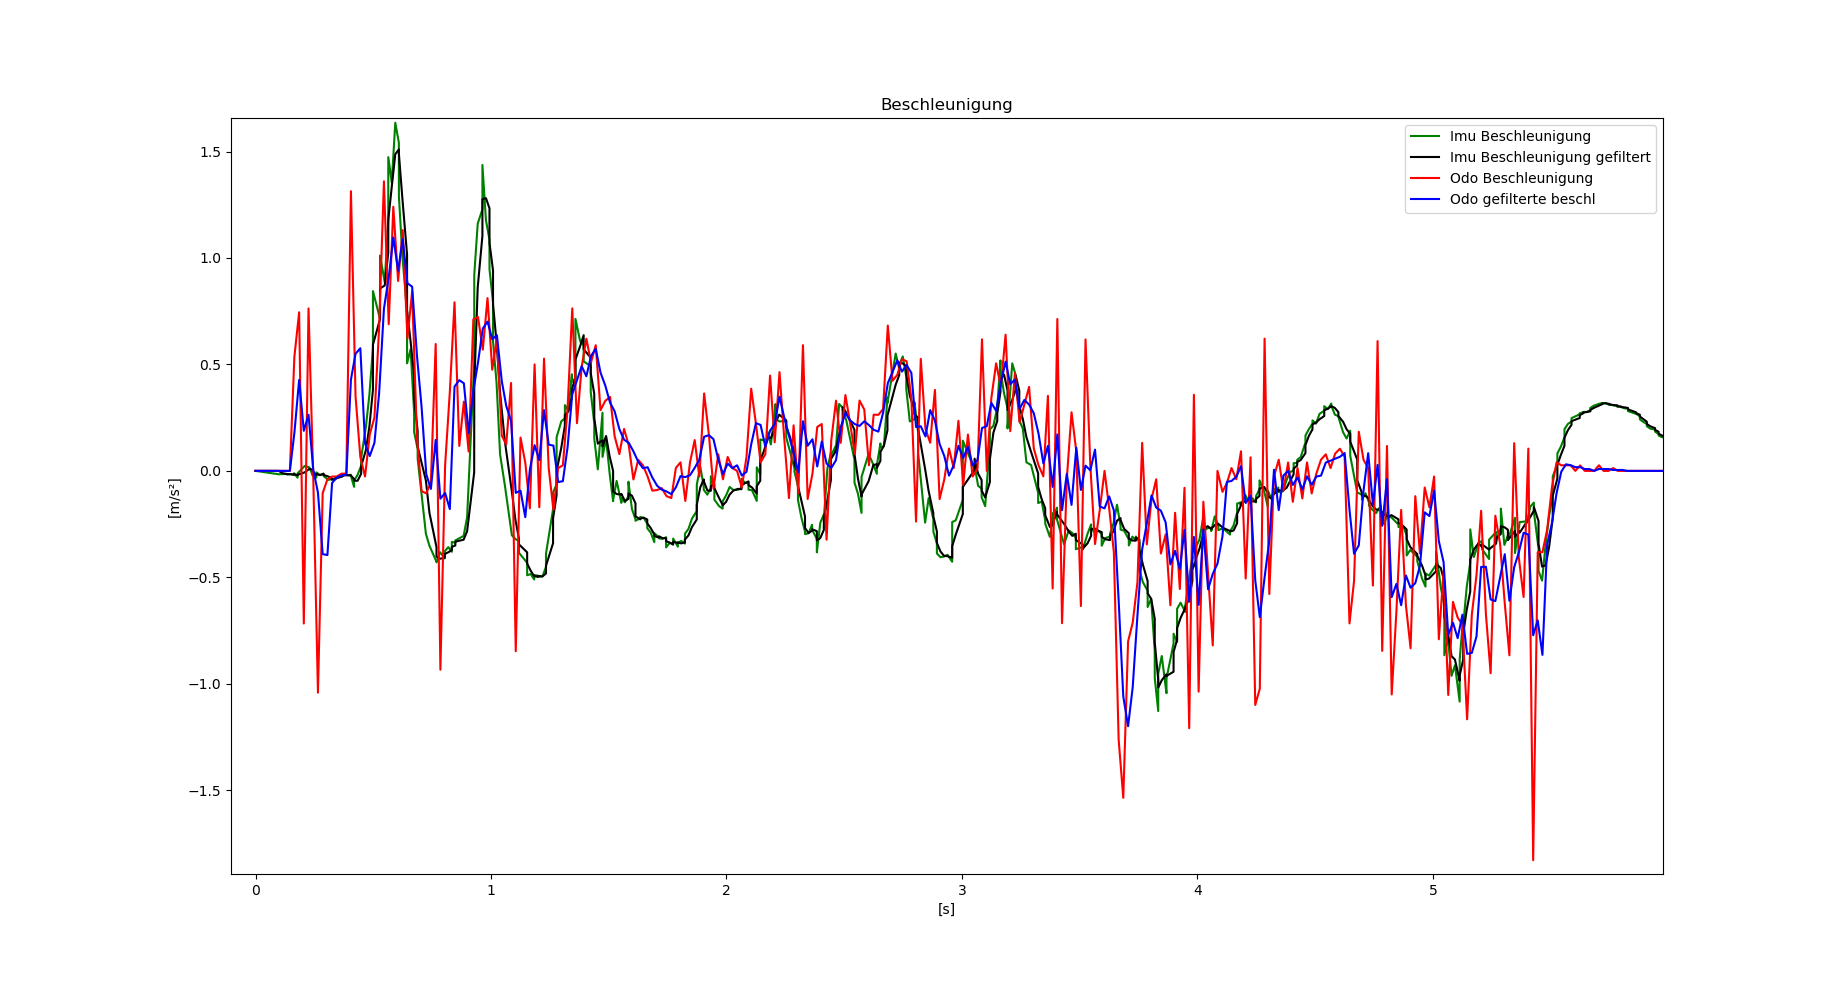
\includegraphics[width=1.2\textwidth]{bilder/23AprBeschlOverlap.png}
    \caption{Beschleunigungswerte übereinander gelegt aktueller Stand}
    \label{fig:diagramApeBeschlOverlap}
\end{figure}



  \clearpage
  %%%%%%
\section{Trajektorienregelung -- Konzeption und Implementierung}
\label{sec:trajektorienregelung}
%

  \clearpage
  %%%%%%
\section{Prototypische Implementierung}
\label{sec:implementierung}
%

  \clearpage
  %%%%%%%
\section{Zusammenfassung und Ausblick}
\label{sec:zusammenfassung}
%



  \clearpage
  \section*{Stichpunkte%
         \label{sec:}}
         
imu (inertia measurement unit):
innere Korrektur-Werte eingestellt (Automatisch Anfang und manuell nachjustiert)
Ziel war es, den Betragsvektor in jeder Orientierung, auf die Größe der Gravitationsbeschleunigung zu bekommen. 

Gesamtziel: Längs und Querdynamic steuerung und regelung. Einschließlich schlupfregelung QUATSCH!!!!

Was bisher geschah:

-Skript geschrieben um den Laptop mit dem Jetson des Autos zu verbinden. (ROS-Master/Slave System)\\
Das dient vor allem dazu, das ich die Skripte auf meinem Laptop ausführen kann was mir schnelleres Arbeiten und das schnelle starten von Tests.

-Skript geschrieben um das Fahrzeug linear zu bewegen. (\lstinline{move_base.py})\\
Dieses Skript wartet auf ein Signal das entweder 0 ist um zu stoppen oder 1 um nach vorne zu fahren in einer bestimmten Geschwindigkeit (Diese ist fix und kann nicht vom Signal übergeben werden). Damit können umfangreiche Tests bezüglich der Beschleunigungs- und Geschwindigkeitsmessung gemacht werden.

-Ein Skript wurde erstellt um die Beschleunigung des resultierenden Vektors zu messen (\lstinline{imuorientation.py})\\
Dieses Skript dient dazu diverse Tests mit der IMU durch zu führen. Durch umfangreiche Versuche wurden so Ungereimtheiten mit der Kalibrierung behoben (Oder eher Verbessert). Hier wird das Topic der IMU abgefangen und einige Zyklen ein Durchschnittswert bestimmt. Der Durchschnittswert soll verhindern das Ausreißer zu viel Einfluss nehmen auf die Tests.

-Zwei Skripte geschrieben um diverse Tests mit der IMU und der Odometrie durch zu führen

    -Einmal wurde das Signal der IMU Integriert um aus der Beschleunigung eine Geschwindigkeit zu bekommen (Hier muss natürlich deutlich mehr Inhalt und Referenzen rein.)
    
    -Zum Schluss wurde das Signal der Odometrie Differenziert um aus der Geschwindigkeit der Odometrie eine Beschleunigung zu bekommen. (Das war analog zum anderen und hat deutlich weniger Aufwand gekostet, könnte natürlich aber auch weiter ausgeführt werden)
    
Zudem musste die IMU Kalibriert werden. Ursprünglich hat die IMU sich mit jedem Neustart selbst Kalibriert, das führte dazu das teilweise die Werte nicht das bestmögliche Resultat lieferten, weshalb wir die IMU getestet haben und die Werte Manuell angepasst haben. (Dieser Vorgang ist noch nicht ganz abgeschlossen da das Ergebnis noch immer nicht ganz Zufriedenstellend ist). 
Das ganze ist notwendig damit die Erdbeschleunigung anschließend sauber raus gerechnet werden kann. Da die IMU sich neigen kann während der Fahrt oder sogar uneben Montiert ist, muss die Erdbeschleunigung raus gerechnet werden um den Drift während des Messens zu minimieren.
Die IMU wurde zudem Software-seitig gedreht mit dem IMU transformer Skript.

Notizen zum 20.04:

IMU Orientierung mit Quaternionen verrechnen um die Erdbeschleunigung zu bekommen. Hierzu wurde das Skript \textbf{imuorientation.py} kopiert und in \textbf{imutests} erweitert um Quaternionen Multiplikation und das bestimmen des Konjugierten Quaternion.
Besonders Hilfreich war dieser \href{https://stackoverflow.com/questions/60492369/gravity-compensation-in-imu-data}{\emph{\textbf{Thread}}}

Die IMU daten werden mit dieser \href{https://docs.ros.org/en/noetic/api/sensor_msgs/html/msg/Imu.html}{\emph{\textbf{Massage}}} Syntax versendet

Mit der Multiplikation von der Ausrichtung als Quaternionen und dem Beschleunigungsvektor kann man die Ausrichtung auf das Erdkoordinatensystem transformieren. Danach ist es möglich den Vektor [0, 0, 9.81] ab zu ziehen und man erhält einen stets bereinigten Sensorwert.

In einem kleinen Test habe ich das ausführlich getestet. Dabei ist raus gekommen das sich der Sensor mittlerweile bis auf zwei Nachkommastellen genau verhält.
Die Werte stehend auf den Rädern auf 4 Nachkommastellen gekürzt.

acc mean: -0.0268 0.0724 -0.0567

roll mean: 1.3763 pitch mean -0.3406 yaw mean: -0.0638

Betrag: 0.0958

Der Betrag weicht immer noch fast ein Zehntel von 0 ab. Das hängt damit zusammen das die Kalibrierung des Sensors noch Abweichungen zu lässt.

Probleme: \\
Es ist derzeit noch ein Problem das nicht der schon bereits gedrehte IMU-Frame genutzt werden kann. Da die Orientierung in diesem nicht geändert wird! Die Frage ist hier ob wir einfach mit dem auf das Erdkoordinaten ausgerichtete System weiter arbeiten können. prinzipiell wäre hier X immer die lineare Bewegung und immer die Querkräfte. 

Weitere nützliche Links:\\
\href{https://stackoverflow.com/questions/39000758/how-to-multiply-two-quaternions-by-python-or-numpy}{\emph{\textbf{Quaternionen Multiplikation in Numpy}}}

Notizen vom 23.04:
\lstinline{imu_gravity_remover} geschrieben. Dieses Script nimmt die daten der IMU und rechnet die Erdbeschleunigung raus. Dieses Skript sendet dann die Daten weiter.
geplant ist das Skript noch in ein cpp skript zu schreiben.

\begin{figure}[H]
  \begin{center}
  
    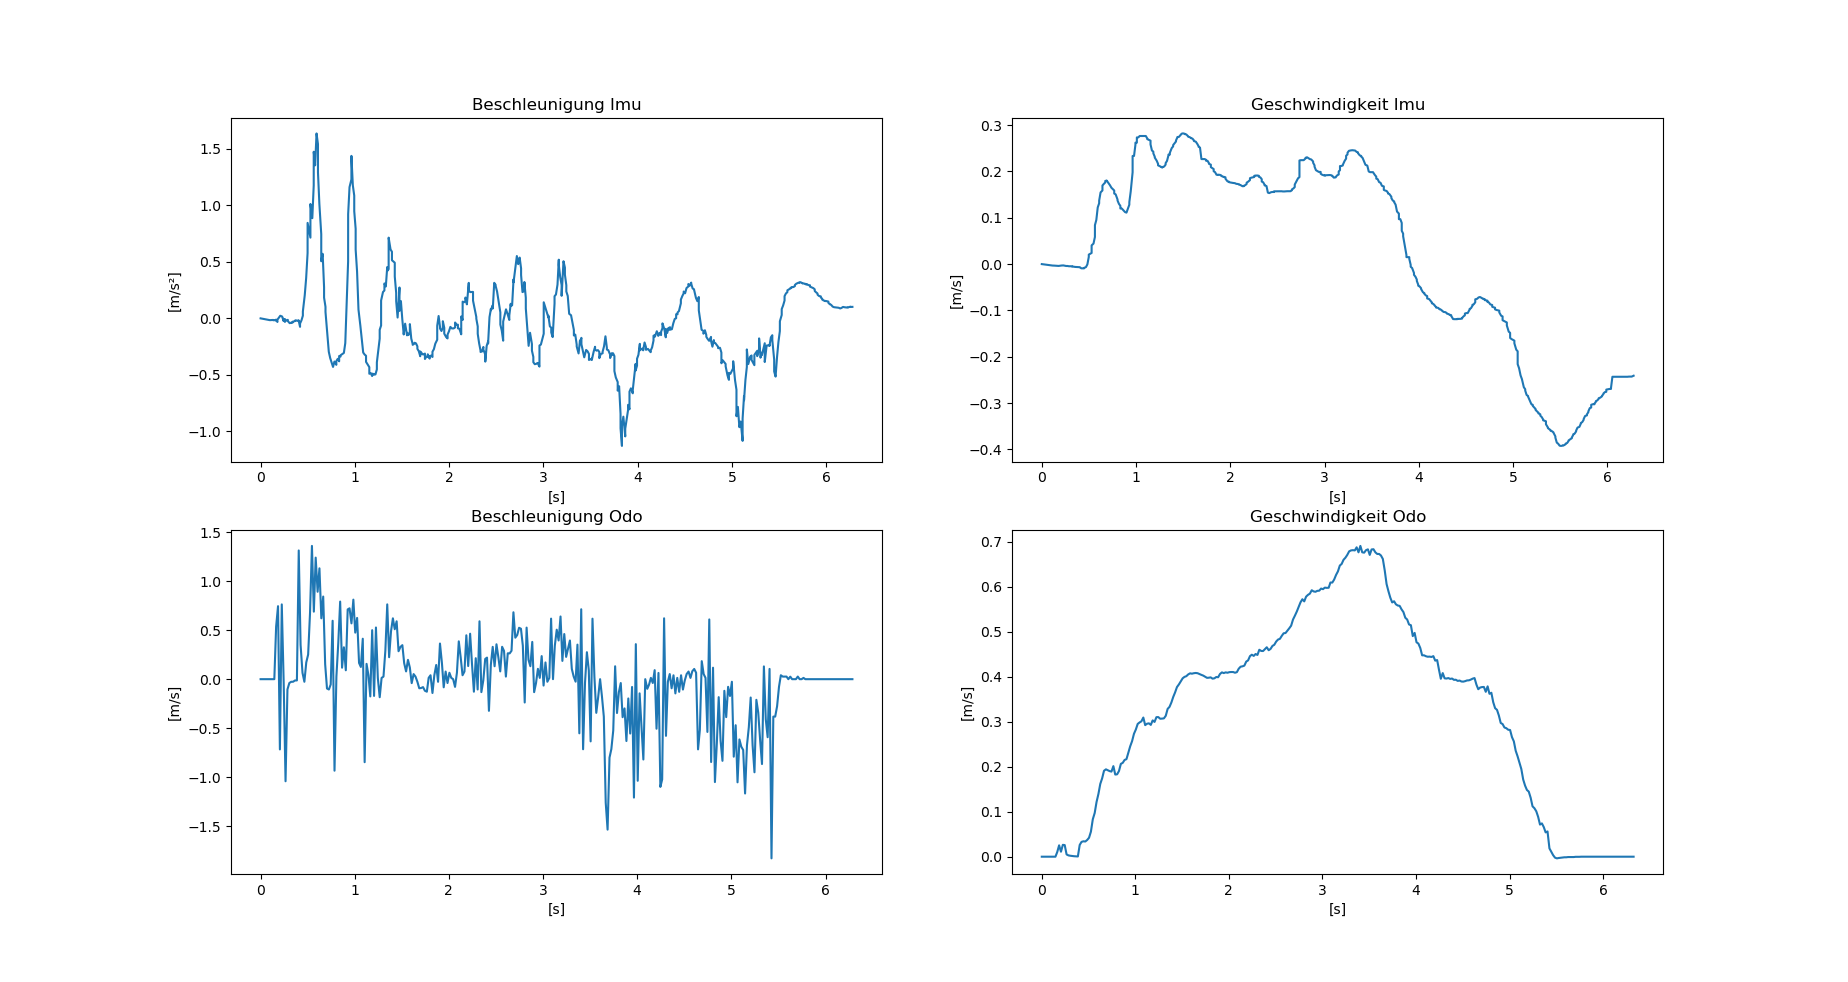
\includegraphics[width=\textwidth]{bilder/23AprImuOdoBeschlGeschw.png}
  \caption{Einzelne Diagramme der Beschleunigung sowie der Geschwindigkeiten}
  \label{fig:diagram1}
  
    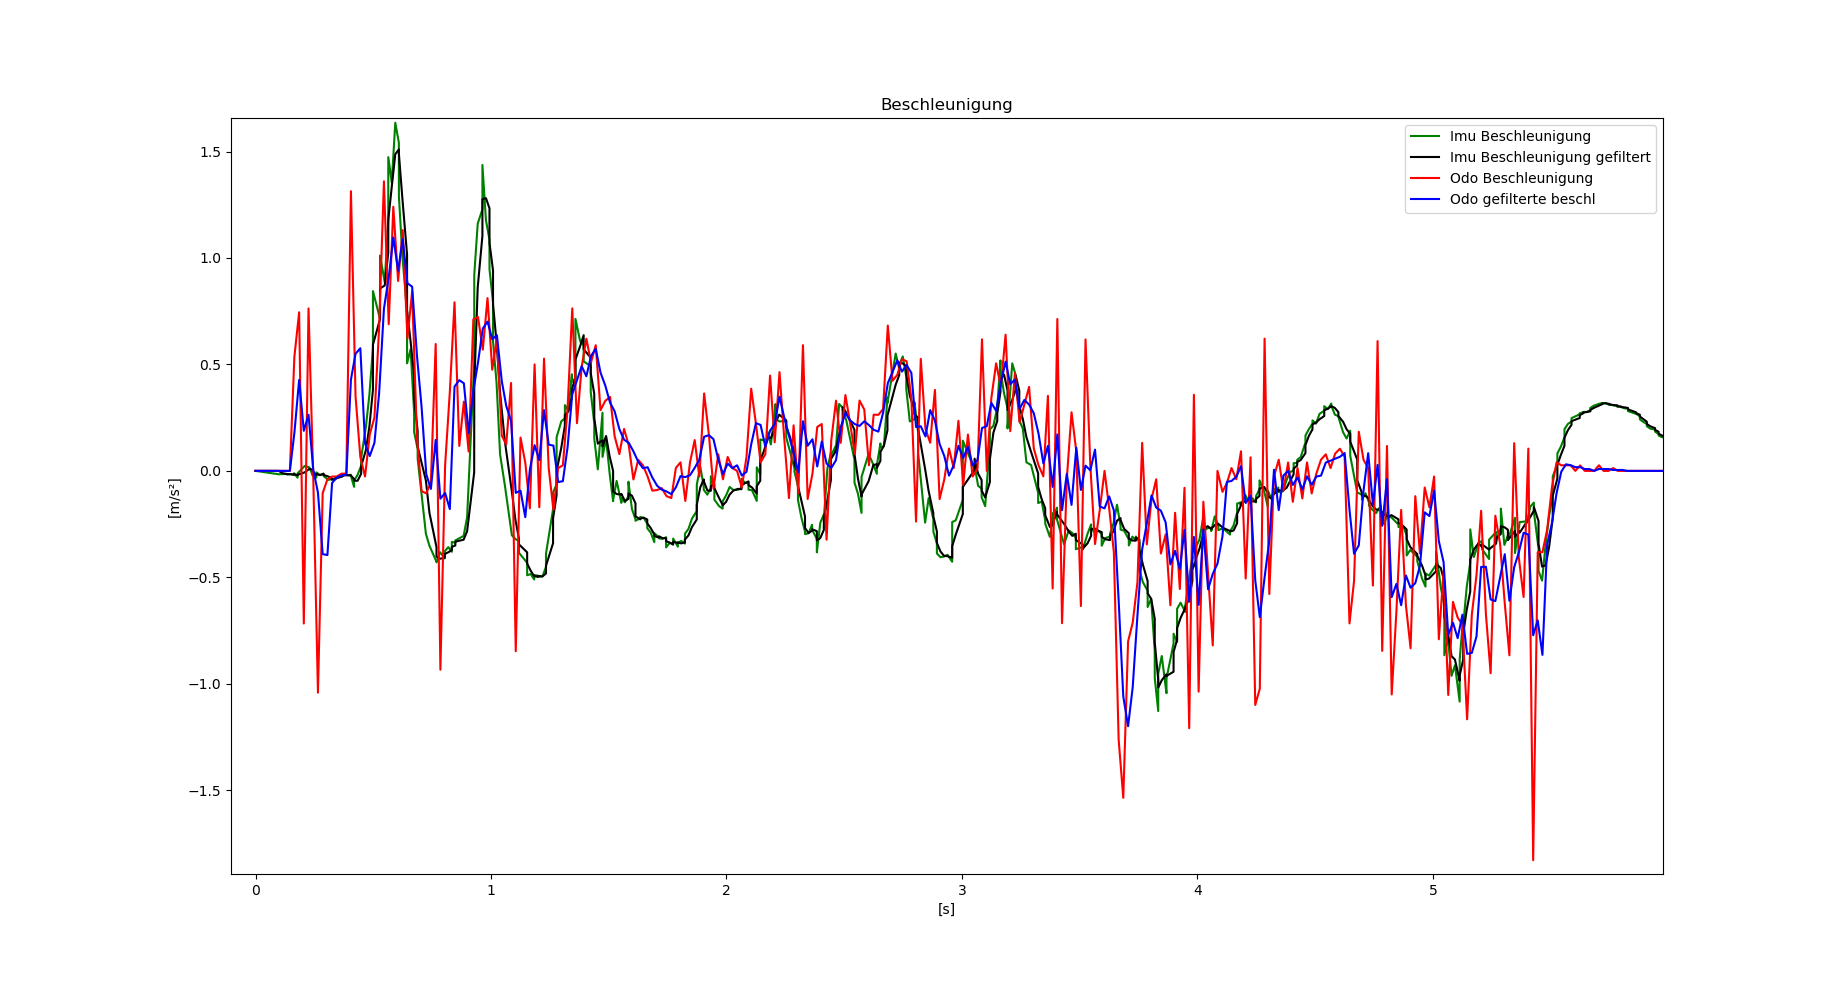
\includegraphics[width=\textwidth]{bilder/23AprBeschlOverlap.png}
  \end{center}
  \caption{Beschleunigungswerte übereinander gelegt aktueller Stand}
  \label{fig:diagram2}
\end{figure}

Wie hier im Bild zu sehen ist, ist das Differenzieren der Odometrie mit recht viel Rauschen verbunden. Im zweiten Diagramm sieht man auch das die Abtastrate sehr ungleichmäßig ist. Derzeit liegt die Vermutung nahe, dass die Skripte nicht schnell genug sind. 
Zudem ist der Drift des Imu immer noch sehr Stark. Die überlegung ist hier mit einem Filter zu arbeiten falls notwendig.

Notizen vom 27.04:
neue Funktion hinzugefügt im \lstinline{cmd_vel_switcher}, um einen Halbautomatischen Modus zu realisieren. Dazu wurden zwei Topics miteinander vermischt und das Signal wieder auf gepublished.

    sec: 1672855594
    nanosec: 699926525
    sec: 1672855594
    nanosec: 715770401
    sec: 1672855594
    nanosec: 731787777
    sec: 1672855594
    nanosec: 731886526
    sec: 1672855594
    nanosec: 747749124
    sec: 1672855594
    nanosec: 764142540
    sec: 1672855594
    nanosec: 764315234
    sec: 1672855594
    nanosec: 779952251


Ausblick dem Arduino das beibringen die Zeit mit zu senden.



 
%  % Abbildungsverzeichnis
%  \clearpage
%  \listoffigures

  % Literaturverzeichnis
  \clearpage
  % manuell in Inhaltsverzeichnis aufnehmen
  \addcontentsline{toc}{section}{Literatur- und Quellenverzeichnis}
%  \addcontentsline{toc}{section}{References}
  % Umbenennen
  \renewcommand\refname{Literatur- und Quellenverzeichnis} % für deutsche Berichte
  % Literaturverzeichnis anzeigen
  \bibliography{hauptdatei}
\clearpage

% 
%. Ggf. Bilderverzeichnis
\listoffigures
\clearpage

%. Ggf. Tabellenverzeichnis
\listoftables
\clearpage

%. Ggf. Abkürzungsverzeichnis
% Steht schon vorne.....

%. Ggf. Stichwortverzeichnis
% Stichwortverzeichnis soll im Inhaltsverzeichnis auftauchen
\addcontentsline{toc}{section}{Stichwortverzeichnis} % für deutsche Berichte
%\addcontentsline{toc}{section}{Index}	% für englische Berichte
% Stichwortverzeichnis endgueltig anzeigen
\printindex
\clearpage


 %%%%%%%%%%%%%%%%%%%%%%%%%%%%%%%%%%%%%%%%%%%%%
  % Anhang
  \clearpage
  \appendix
  \addcontentsline{toc}{section}{Anhang} % Für deutsche Berichte 
%  \addcontentsline{toc}{section}{Appendix}	% für englische Berichte 
  % Formatierung des Anhangs
  % Bildnummern aus Nummer des Abschnitts und laufender Nummer zusammensetzen
  %
  % Bei Verwendung eines Bericht-Formats (s.o.) geschieht dies
  % automatisch mit der Kapitelnummer (\chapter – eine Ebene oberhalb
  % von \section). Für das Artikel-Format machen wir es hier manuell.
  %
  \renewcommand{\thefigure}{\Alph{section}.\arabic{figure}}
  \makeatletter\@addtoreset{figure}{section}\makeatother
  % Gleichungsnummern aus Nummer des Abschnitts und laufender Nummer zusammensetzen
  \renewcommand{\theequation}{\Alph{section}.\arabic{equation}}
  \makeatletter\@addtoreset{equation}{section}\makeatother
  % Tabellennummern aus Nummer des Abschnitts und laufender Nummer zusammensetzen
  \renewcommand{\thetable}{\Alph{section}.\arabic{table}}
  \makeatletter\@addtoreset{table}{section}\makeatother
  %%%%
  % Inhalt des Anhangs
  % Anhang A
\section{Fertigungszeichnungen}









  % Eidesstattliche Erklärung
  \clearpage
  \fancyhead[L]{Eidesstattliche Erklärung} % Kopfzeile links
  %\addcontentsline{toc}{section}{Eidesstattliche Erklärung}
  %%%%%%%%%%%%%%%%%%%
\section*{Eidesstattliche Erklärung}
%
Ich versichere, dass ich die Arbeit selbständig verfasst und keinen als die angegebenen Quellen und Hilfsmittel benutzt sowie Zitate kenntlich gemacht habe. 
%
\bigskip 

Die Regelungen der geltenden Prüfungsordnung zu Versäumnis, Rücktritt, Täuschung und Ordnungsverstoß habe ich zur Kenntnis genommen. 
%
\bigskip

Diese Arbeit hat in gleicher oder ähnlicher Form keiner Prüfungsbehörde vorgelegen. 
%
\bigskip 

%Ich versichere, die von mir vorgelegte Arbeit selbstständig verfasst zu haben.
%Alle Stellen, die wörtlich oder sinngemäß aus veröffentlichten oder nicht veröffentlichten 
%Arbeiten anderer entnommen sind, 
%habe ich als entnommen kenntlich gemacht. 
%Sämtliche Quellen und Hilfsmittel, die ich für die Arbeit benutzt habe, sind angegeben. 
%Die Arbeit hat mit gleichem Inhalt bzw. in wesentlichen Teilen noch keiner anderen Prüfungsbehörde vorgelegen.
%

\vspace{3cm}
Heiligenhaus, den 
\underline{\hspace*{3cm}}
\hfill 
\begin{tabular}[t]{@{}l@{}}\hline
\hspace*{2.5cm}Unterschrift\hspace*{2.5cm}
\end{tabular}


\end{document}
